% Put labels, etc., on figures using PSTricks.
% Use dvips -E <file>.dvi -o <file>.eps to create encapsulated PostScript.
%
\documentclass[12pt]{article}
\usepackage{graphicx}
\usepackage{pstricks}
\pagestyle{empty}

\begin{document}
\rput(5,-5){
\rput(.1,-.1){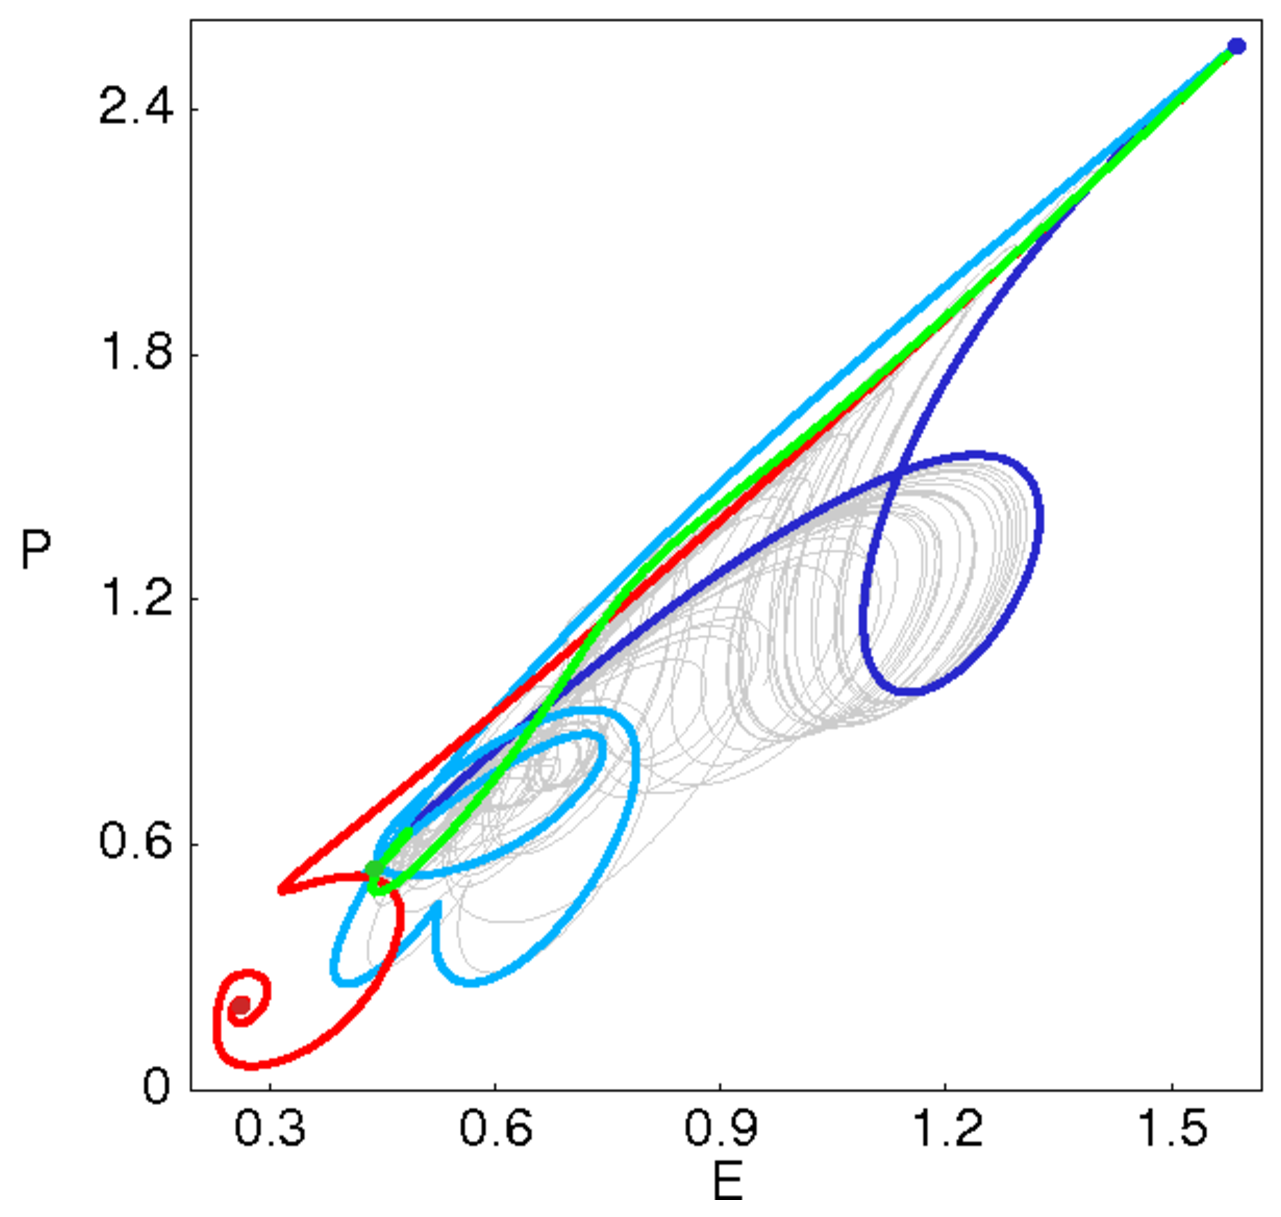
\includegraphics{../../figs/connEP.eps}}

\huge

% \psframe*[linecolor=white](-6.5,6)(-5.5,7)
% \psframe*[linecolor=white](6,-6.5)(7.2,-5.5)

\rput(10.1,8.3){E$_3$} 

\psline[linewidth=2pt]{->}(-7,-5.5)(-6.7,-6.7)\rput(-7,-5){E$_1$}

\psline[linewidth=2pt]{->}(-5.8,-3.65)(-4.5,-4.5)\rput(-6.3,-3.55){E$_2$}
\psline[linewidth=2pt]{->}(4.5,-5)(2,-2.7)\rput(4.5,-5.5){``Turbulence''}


% Use grid command below to place objects at specified coordinates.
%  \psgrid[subgriddiv=1,griddots=10](-8,-8)(10,10)
}
\end{document}
